\documentclass{article}
\usepackage{graphicx}
\usepackage{hyperref}
\usepackage{amsmath}
\usepackage[a4paper, total={6in, 8in}]{geometry}

\begin{document}

\begin{titlepage}
    \begin{center}
        \vspace*{1cm}
            
        \Huge
        \textbf{Electricity Usage Optimizer}
            
        \vspace{0.5cm}
        \LARGE
        Miniproject Report
        
        \date{today}
            
        \vspace{1.5cm}
            
        Pontus Hedlund, Sanna Korpi, Topi Ranta
            
        \vfill
            

            
        \vspace{0.8cm}
            
            
        \Large
        University of Helsinki\\
        Introduction to Data Science\\
        31.10.2022\\
            
    \end{center}
\end{titlepage}

\tableofcontents

\vspace{30.0 cm}

\section{A Simple Prediction of Electricity Price Development}
\label{section:introduction}

This report describes technical aspects of an electricity price prediction software made as Introduction to Data Science course mini project. The estimation tool is a Python web application that provides a 36-hour electricity price development prediction based on a model trained with \href{https://xgboost.ai/}{XGBoost library}. The forecast is shown as an hourly three-step recommendation scale and it is based on a linear regression model trained using historical data including electricity price, wind power, power consumption and weather data.

The report includes references to \href{https://github.com/IDS-mini/electricity}{the project repository in Github}. In addition to the data exploration, the regression model and the web application source code, the repository also includes our \href{https://github.com/IDS-mini/electricity/blob/main/marketing/Mini-Project-Canvas-Hedlund-Korpi-Ranta.pdf}{project canvas}, \href{https://github.com/IDS-mini/electricity/blob/main/marketing/presentation.pptx}{product pitch presentation} and \href{https://github.com/IDS-mini/electricity/blob/main/src/app/templates/index.html}{web application home page}. As this report does not discuss the added value or the business side of the project, it is advisable to walk through those documents before reading this technical report.

The rest of the report is composed as follows: the data used and data preprocessing are described in Chapter \ref{section:data}. The prediction formulation and the linear regression model used in the project are reported in Chapter \ref{section:analysis}. User experience and results delivery for the end user are displayed in Chapter \ref{section:delivery}. Observations, discussion and ideas for further development are presented in \ref{section:conclusions}.

\section{Data}
\label{section:data}

In order to produce the prediction, several sets of historical data were used. The data sets are described in Subchapter \ref{subsection:datadescription} and comments on the data exploration and preprocessing in Subchapter \ref{subsection:eda}. Data storage and protection are reported in Subchapter \ref{subsection:warehousing}.

\subsection{Data Used in the Project}
\label{subsection:datadescription}

%% why this data, ref to feature extraction

The data sources used in the project are \href{https://data.fingrid.fi/en}{Fingrid Wind Power Production and Total Consumption Data}, \href{https://transparency.entsoe.eu}{Entsoe Day-ahead Market Price Data}, \href{https://en.ilmatieteenlaitos.fi/open-data}{Finnish Meteorological Institute Weather Observation Data for Kumpula, Helsinki}. The data was accessed in two ways. Large, historical data sets were manually downloaded for exploration, feature extraction and model training and programmatic access was used to enable the web application to get the latest data for user predictions. The programmatic access includes API connections and web scraping.

Even though all the data is available for free, some sources require registering an account to download the full data or access most recent data via API. Characteristics of the data sources are presented in Table \ref{table:source-characteristics}.

\begin{table}[ht] 
\centering 
\begin{tabular}{l||l c c} 
data set & Format & Access via & Registration\\ 
\hline \hline
Entsoe & CSV & UIM, WS  & Required for full history access \\
FMI & CSV & UI, API & Not required \\
Fingrid & CSV & UIM, API & Required for API access \\
\hline
\end{tabular}
\caption{The data sources used in the project. UIM is abbreviation for manual download via user interface and WS for web scraping.}
\label{table:source-characteristics}
\end{table}

Entsoe Day-ahead Prices data consists of hourly electricity market prices for Finnish Bidding Zone that covers the whole country. \href{https://data.fingrid.fi/en/data set/wind-power-generation}{The Wind Power Production} data set includes hourly wind power production in Finland in $MWh/h$, \href{https://data.fingrid.fi/en/data set/electricity-consumption-in-finland}{Electricity Consumption} data set $MWh/h$ consumption and from \href{https://en.ilmatieteenlaitos.fi/open-data}{Weather Data} we picked air pressure, rain, humidity, temperature and wind. \href{https://www.helen.fi/en/company/responsibility/current-topics/open-data}{Helen District Heating Power Data} was investigated but was reject, as the data was only available until the end of year 2021.

All the data used in project is provided in one hour interval thus making data integration rather easy. The historical data was downloaded spanning from the beginning of 2019 as far ahead as possible. Beginning of 2019 was chosen so that the current volatile prices would not be marginalized in the data set. A visualization of 2022 price volatility can be viewed in Figure \ref{fig:prices-history}.

\begin{figure}[ht] 
\centering
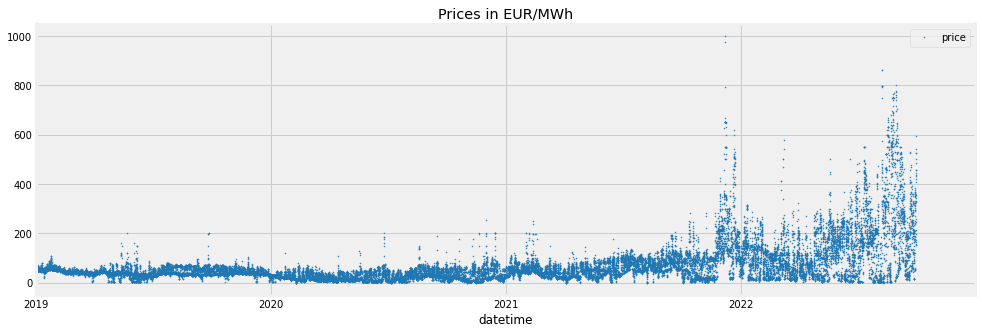
\includegraphics[width=\textwidth]{report/images/day-ahead-prices.png}
\caption{Day-ahead market prices for electricity in Finland.}
\label{fig:prices-history} 
\end{figure}

\subsection{Exploratory Data Analysis and Data Preprocessing}
\label{subsection:eda}

The purpose of the exploratory data analysis (EDA) and data preprocessing phase was to understand the data and its possible shortages and produce an integrated data set for model training with missing values imputed. This phase was conducted in series of Jupyter Notebook files. The cleaned csv files were written into Apache Parquet format for better data compression and reading performance before integration. The eda and data cleaning notebooks are listed in Table \ref{table:eda}.

As expected, the data cleaning and integration was rather effortless. Missing data rates were low (for example, less than 0.4\% day-ahead prices were missing) and missing values imputation was performed using neighbor values, which intuitively works well with time-series data. In the cleaning process, datetime column was set as data set as index and was thus later used as key to integrate the cleaned parquet files.

\begin{table}[ht] 
\centering 
\begin{tabular}{l||l c} 
Data set & Imputation method & File\\ 
\hline \hline
Day-ahead & Previous neighbor & \href{https://github.com/IDS-mini/electricity/blob/main/data/day-ahead_clean.ipynb}{day-ahead\_clean.ipynb},  \href{https://github.com/IDS-mini/electricity/blob/main/data/day-ahead_eda.ipynb}{day-ahead\_eda.ipynb}\\
Consumption & - & \href{https://github.com/IDS-mini/electricity/blob/main/data/consumption_eda.ipynb}{consumption\_eda.ipynb} \\
Weather & Neighbor values mean & \href{https://github.com/IDS-mini/electricity/blob/main/data/weather_eda.ipynb}{weather\_eda.ipynb} \\
Wind power & - & \href{https://github.com/IDS-mini/electricity/blob/main/data/wind_power_eda.ipynb}{wind\_power\_eda.ipynb}\\
\hline
\end{tabular}
\caption{The data sets used to train the model. Links to data sets' EDA Jupyter notebook files are presented in the File column.}
\label{table:eda}
\end{table}

In addition to the cleaned historical data, time series forecasts for each data sets were created. The former were used to train the model and the latter, supplemented with latest data renewed via programmatic data fetching, to construct final predicted price. The data was integrated in \href{https://github.com/IDS-mini/electricity/blob/main/data/data_integration.ipynb}{data\_integration.ipynb} where new features were also extracted. Both feature extraction and prediction creation process are further discussed in Chapter \ref{section:analysis}.

%% eda findings

    %% week and day cycle of electricity price
    %% cold weather effecting consumption
    %% connection between consumption and price

\subsection{Data Warehousing and Data Protection}
\label{subsection:warehousing}

Both the raw, manually downloaded data and the cleaned data were stored in the project repository. As datasets were reasonably-sized, data files being around 0.5 MB, the code repository solution was seen to be adequate. Larger project would have required a more scalable warehousing solution, for example a cloud-based blob storage.

All data used in our project is publicly available and does not include any personal data, so no data used in the project was subject to the GDPR act. Therefore, the warehousing solution's sole purpose was to share the data changes and cleanings between project developers and to keep the data backed up and version controlled.

\section{Data Analysis}
\label{section:analysis}

The purpose of the project and the data analysis was to create a 36-hour estimate on electricity hourly market price development. In order to do so, new features were extracted from the cleansed and integrated data, scripts for refreshing the data were written and supplementary predictions made. The feature extraction is reported in Subchapter \ref{subsection:extraction}, training the XGBoost Regressor is presented in Subchapter \ref{subsection:xgboost} and data refreshing and intermediate forecasts to support contemporary predictions are discussed in Subchapter \ref{subsection:datafilling} .

\subsection{Feature Extraction}
\label{subsection:extraction}

%% time series features

First, we extracted new features from datetime index itself. As electricity usage and thus market price fluctuations are cyclic and depend on time of the year, the datetime was decomposed to several new features. A rather intuitive example of how these features might affect the rest of the data components is illustrated in Figure \ref{fig:components}.

\begin{figure}[ht] 
\centering
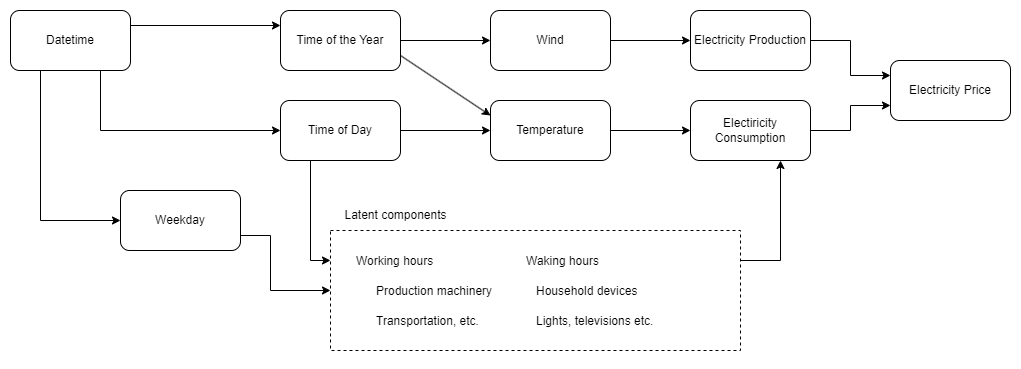
\includegraphics[width=\textwidth]{report/images/components.png}
\caption{A simplified diagram on how we assumed different components could affect each other and thus the target value.}
\label{fig:components} 
\end{figure}

%% lag features


\subsection{Time Series Prediction with XGBoost}
\label{subsection:xgboost}

%% data set to train the model, table

Features extracted for the model were:

'WindMWh', 'ConsumptionMWh', 'pressure', 'rain', 'humidity',

'temperature', 'wind' and the target value was 'price'.

The ML model used for this application is the XGBoost Regressor, which is an ensemble method based on gradient-boosted decision trees. It was found to be very fast to train and very accurate.

When training the models, we used cross validation with time series splits (See figure \ref{fig:ts-cross-validation}). 

The forecast is done twice a day with Github actions and saved to the repository. The webapp shows the latest forecast.

\begin{figure}
    \centering
    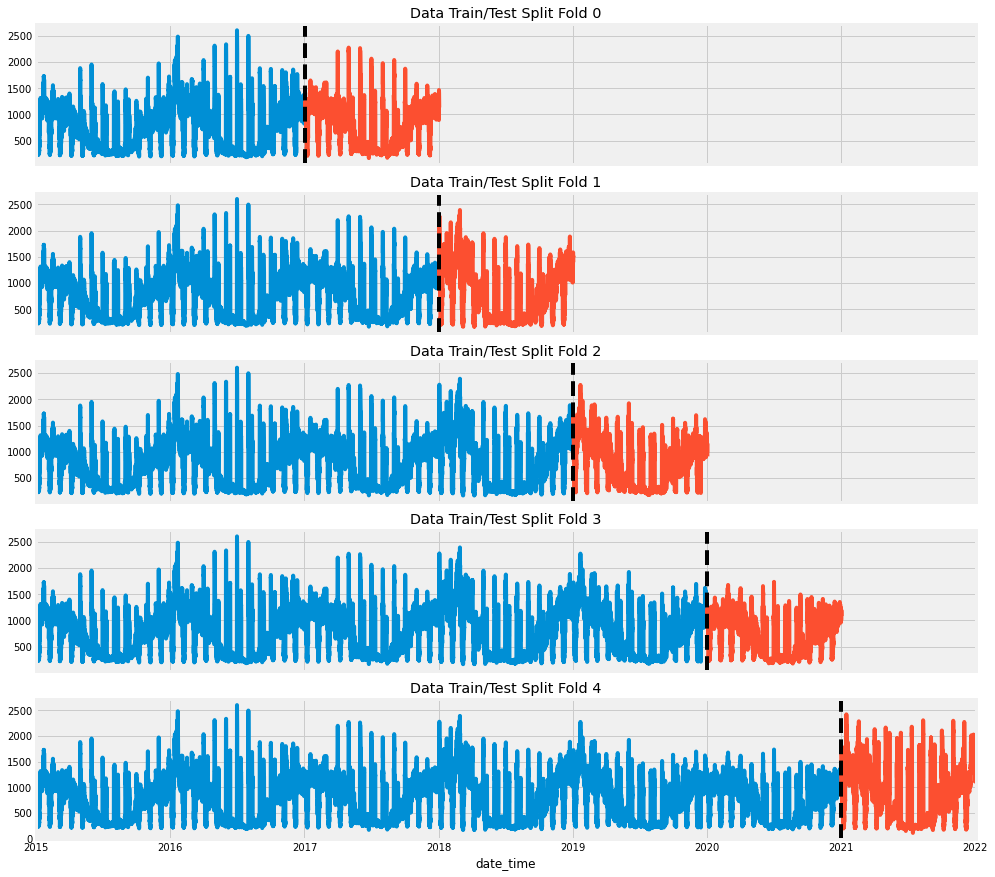
\includegraphics[width=15cm]{report/images/ts-cross-validation.png}
    \caption{Cross validation using Time Series Splits with each split being a year.}
    \label{fig:ts-cross-validation}
\end{figure}

\subsection{Gathering the Data for the Prediction}
\label{subsection:datafilling}

Since the model is trained on past data, all the same variables need to be present when performing the prediction. Since all of these are not available for the prediction time, we created time series forecasts as a base that should give a best estimate of the values (See figure \ref{fig:consumption}). Then if newer data was available, this forecasted base was updated through programmatic data fetching.

\begin{figure}
    \centering
    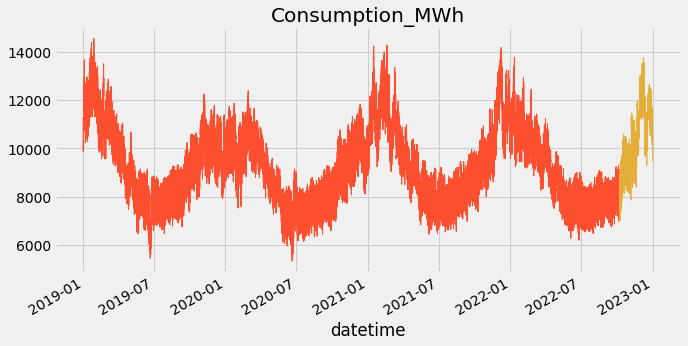
\includegraphics[width=15cm]{report/images/consumption.png}
    \caption{Time series for Consumption in MWh with historical data in red and the forecast in orange.}
    \label{fig:consumption}
\end{figure}





\section{Delivering Results for the End User}
\label{section:delivery}

We calculate a simple moving average (SMA) of the electricity price with a window of 168 hours (7 days) to create a reference price point. For each prediction time, we compare the predicted or known price to the index via equation \ref{eq:index}.


\begin{equation} \label{eq:index}
\text{"Price Index"}_i = \frac{\text{SMA}_i}{\text{"Predicted Price"}_i}
\end{equation}

The price index is then classified as follows:

\begin{enumerate}
    \item $\text{"Price Index"}_i < 0.8$ : "Boost"
    \item $0.8 \leq \text{"Price Index"}_i \leq 1.2$ : "Maintain"
    \item $\text{"Price Index"}_i > 1.2$ : "Restrict"
\end{enumerate}

\subsection{Web Application}
\label{subsection:server}

Our deliverable is a web application built with FastAPI that serves a landing page and a page for planning. The plan page shows a table with hourly times for the next 36 hours with a recommendation and the price index. The whole package is available on Github at https://github.com/IDS-mini/electricity .

\subsection{Visualization and User Experience}
\label{subsection:ux}

%% no gdpr data gathered from the user either

\section{Conclusions}
\label{section:conclusions}

%% what was achieved
%% what was learned
%% what we would do differently
%% ideas for further development or research


\end{document}

